
%%%%%%%%%%%%%%%%%%%%%%%%%%%%%%%%%%%
\chapter{Introduction}
\label{ch:introduction}
%%%%%%%%%%%%%%%%%%%%%%%%%%%%%%%%%%%
	Over the past century humanity has become increasingly dependent on the 4th state of matter, plasma. Attaining a better understanding of plasma behavior and interaction is critical to developing faster computer chips, creating new sources of energy, and expanding humanities influence amoung the stars. One important subset of plasma behaviour is how plasmas interact with solid objects such as dust particles, probes, and bodies traveling through space. These interactions can be very difficult to explore experimentally, and therefore must be modelled. 
	
A plasma's behaviour is heavily influenced by the collective electric and magnetic fields generated by the individual particles that comprise the plasma. This means that plasma behaviour is essentially a very large n-body problem, where for moderately dense plasmas n can be on the order of $10^{20}$. No computer currently in existence can store the information for $10^{20}$ particles, and calculating the interaction of every particle in the set with every other particle would be prohibitvely long. The solution to this problem is to model only a subset of the true number of particles. The modeled behaviour of these particles and their contributions to magnetic and electric fields can be used to statistically infer the behaviour of the rest of the plasma, essentially from first princeiples. This method is called particle-in-cell (PIC), and operates by moving particles on a potential grid and updating that potential with the new particle density at every timestep. The flow of a general PIC code is shown in figure \ref{fig:pic_flowchart}. The PIC method is a very robust and straightforward scheme for modeling plasma behaviour, and is used extensively to model plasmas in complicated systems.

\begin{figure}
\begin{center}
%\documentclass[a4paper,5pt]{article}
%\usepackage{tikz}
%\usetikzlibrary{arrows,positioning} 


%\begin{document}

\noindent
\begin{tikzpicture}[node distance=1cm,font=\footnotesize,auto]
\tikzset{
    %Define standard arrow tip
    >=stealth',
    %Define style for boxes
    punkt/.style={
           rectangle,
           rounded corners,
           draw=none, very thick,
           text width=2.5cm,
			  minimum width=2.6cm,
           minimum height=1.5cm,
			  },
    % Define arrow style
    pil/.style={
           ->,
           very thick,
           shorten <=2pt,
           shorten >=2pt,},
    punkt2/.style={
           rectangle,
           rounded corners,
           draw=black, very thick,
			  minimum width=2.65cm,
           minimum height=1.35cm,
			  anchor=west},
    punkt3/.style={
           rectangle,
           rounded corners=15pt,
           draw=black,
			  minimum width=3.2cm,
           minimum height=2.0cm,
			  }
}
	\noindent
 	\node[shift={(0cm,0cm)}] (dtcenter) at (0,0) {$\Delta t$};
	\node[shift={(160:1cm)}] (circstart) at (dtcenter) {};
	\draw[pil] (circstart) arc (160:-160:1cm);
 %nodes

 	\node[punkt,shift={(-2.5cm,2.5cm)}] (padvnc2) at (dtcenter) {Integrate equations of motion\newline $\mathbf{F}_i \rightarrow \mathbf{v}_i' \rightarrow \mathbf{x}_i$};

 	\node[punkt,shift={(2.5cm,2.5cm)}] (ploss2) at (dtcenter) {Particle loss and re-injection};

	\node[punkt,shift={(7.0cm,0)}] (collide2) at (dtcenter) {Monte Carlo collisions\newline $\mathbf{v}_i' \rightarrow \mathbf{v}_i$};

	\node[punkt,shift={(2.5cm,-2.5)}] (c2mesh2) at (dtcenter) {Interpolate particles to mesh\newline $(\mathbf{x}_i,\mathbf{v}_i) \rightarrow \rho_j$};

	\node[punkt,shift={(-2.5cm,-2.5)}] (psolve2) at (dtcenter) {Integrate field equations\newline $\rho_j \rightarrow \mathbf{E}_j$};

	\node[punkt,shift={(-5.5cm,0)}] (mesh2p2) at (dtcenter) {Interpolate field to particles\newline $\mathbf{E}_j \rightarrow \mathbf{F}_i$};

	\node[punkt2] (padvnc) at (padvnc2.west) {};
	\node[punkt2] (ploss) at (ploss2.west) {};
	\node[punkt2] (collide) at (collide2.west) {};
	\node[punkt2] (c2mesh) at (c2mesh2.west) {};
	\node[punkt2] (psolve) at (psolve2.west) {};
	\node[punkt2] (mesh2p) at (mesh2p2.west) {};

	\path (padvnc.east) edge[pil] (ploss.west);
	\path (ploss.east) edge[very thick,dashed,out=-60, in=60,shorten <=2pt,shorten >=2pt,] (c2mesh.east);
	\path (ploss.east) edge[pil,out=0, in=90] (collide.north);
	\path (collide.south) edge[pil,out=-90, in=0] (c2mesh.east);
	\path (c2mesh.west) edge[pil] (psolve.east);
	\path (psolve.west) edge[pil,out=180,in=-90] (mesh2p.south);
	\path (mesh2p.north) edge[pil,out=90,in=180] (padvnc.west);
	

\end{tikzpicture}


%\end{document}

%%% Local Variables:
%%% mode: latex
%%% TeX-master: t
%%% End:

\end{center}
\caption{Flow schematic for the PIC method.}
\label{fig:pic_flowchart}
\end{figure}


%%%%%%%%%%%%%%%%%%%%%%%%%%%%%%%%%%%% 
	\section{Motivation}
%%%%%%%%%%%%%%%%%%%%%%%%%%%%%%%%%%%%

	The PIC method is very good at modeling complicated plasma behaviour, however this method still relies on tracking a very large number of particles for good statistics. In order to achieve ``good'' statistics PIC codes employ millions to billions of particles, which means that these codes can require a very large amount of computation time for each timestep. Running millions of particles on a single processor for hundreds of timesteps is not really feasible, it simply takes too long to compute a solution. 
	
	One way to reduce the total run time of PIC codes is to parallelize them. Since PIC codes operate on the fact that the potential changes little over the course of a single timestep, each particle can be assumed to be independent of its neighbors. This leads to a situation that is trivially parallel. In theory a machine with a million processors could run every particle on a seperate processor. This is of course assuming that the majority of the computational complexity lies in moving the particles and that comunication between processors is very fast.  


%%%%%%%%%%%%%%%%%%%%%%%%%%%%%%%%%%%%
		\subsection{GPUs vs CPUs}
%%%%%%%%%%%%%%%%%%%%%%%%%%%%%%%%%%%%
	The ideal computing system for a particle in cell code should have a large number of relatively simple processors with very low communication costs. Traditional CPUs are just the opposite of this. CPUs tend to have 4-8 complicated processors that are very good at performing large operations on small sets of data, but very slow when it comes to communicating between multiple processors. CPUs are designed to be able to actively switch tasks on the fly. This makes them very good at simultaneously running web-browser, decoding a video, and playing a video game. However, this flexibility requires a large number of cycles to switch between tasks, and a large amount of cache to store partially completed tasks.

Graphical processing units, or GPUs, forgo the flexibility of CPUs in favor of more raw processing capability. Reducing the size of the cache and employing single instruction multiple data (SIMD) parallelism allows GPU manufactures to combine hundreds of processors on a single chip. In order to supply enough data to keep hundreds of processors GPUs also have a very large data channel between the processors and DRAM. All of these features are chosen to create a math processor that excels at tasks where each processor operates on data that is invisible to the other processors. These features give GPUs a significant raw floating point performance advantage over CPUs as seen in figure \ref{fig:gpu_vs_cpu}. 


\begin{figure}
\begin{center}
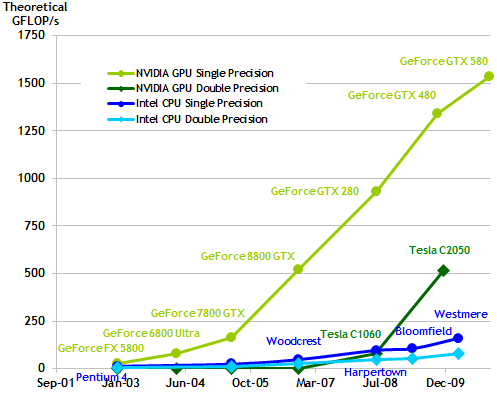
\includegraphics[width=5in]{introduction/gpu_vs_cpu.png}
\end{center}
\caption{Performance comparison of GPUs vs CPUs.}
\label{fig:gpu_vs_cpu}
\end{figure}

The hardware in GPUs is tailored to excel at performing tasks such as ray-tracing, which is very similar to particle moving. Therefore it is by no means unreasonable to conclude that GPUs can be very good PIC code processors. The advantages that GPUs have over CPUs for scientific computing include:

\begin{itemize}
	\item Higher performance per cost.
	\item Higher performance per watt.
	\item Easier to upgrade.
	\item GPUs still improving with Moore's law.
\end{itemize}

All of which are observed when comparing the CPU and GPU versions of the same PIC code. While these advantages are very promising there are also several disadvantages to GPU computing:

\begin{itemize}
	\item Increased code complexity.
	\item Smaller memory space.
	\item Smaller cache.
	\item Slow communication between CPU and GPU.
	\item Most developed GPU language is an extension of C.
	\item Algorithms can be very dependent on hardware configuration.
\end{itemize}

The key to developing efficient PIC algorithms that utilize GPUs lies in balancing the work between the two architectures. Some operations will be easier to implement on the CPU and be just as fast as the GPU while others will be significantly faster on the GPU. Partitioning the code between the different architectures begins to outline a very important aspect of parallel computing, multiple levels of parallelism.

%%%%%%%%%%%%%%%%%%%%%%%%%%%%%%%%%%%%
	\section{Multiple Levels of Parallelism}
%%%%%%%%%%%%%%%%%%%%%%%%%%%%%%%%%%%%
	Currently most parallelization is done by dividing up a task between a bunch of threads on different CPUs, and using an interface such as MPI to allow those threads to communicate. This network of threads has a master node, usually node 0, which orchestrates the communication between the other nodes. This is analogous to how a single CPU-GPU system operates. The CPU is the ``Master'' and serves as a communication hub for groups of execution threads on the GPU called thread blocks. Each thread block is itself a cluster of threads that can communicate through a memory space aptly named ``shared memory''.

\begin{figure}
\begin{center}
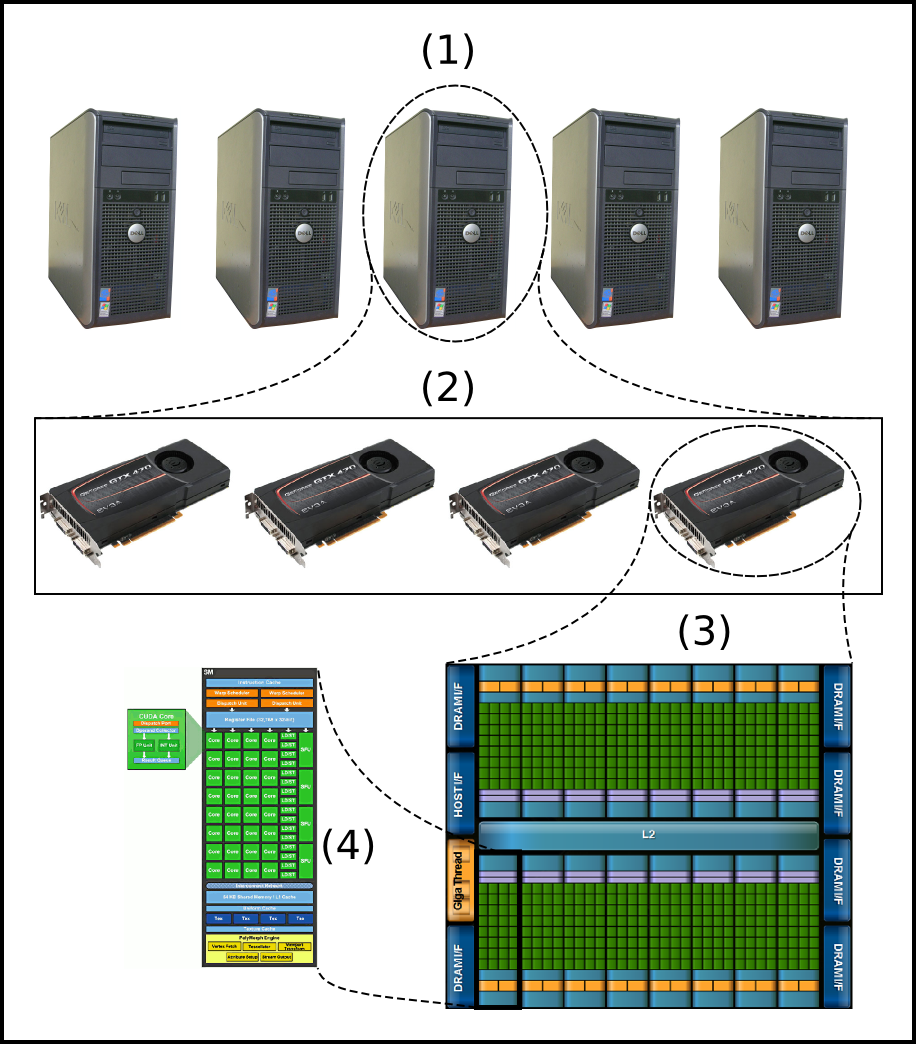
\includegraphics[width=5in]{introduction/multi_parallel.png}
\end{center}
\caption{Multiple levels of parallelism. (1) Cluster of systems communicating through a LAN. (2) Multiple GPUs per system communicating through system DRAM. (3) Multiple streaming multiprocessors per GPU execute thread-blocks and communicate through GPU global memory. (4) Multiple cuda cores per multiprocessor execute thread-warps and communicate through on chip shared memory. }
\label{fig:multiparallel}
\end{figure}

The point hear is that multiple domain decompositions must be performed in order to fully utilize the capabilities of this system. The coarse decomposition is very similar to that used for MPI systems, but the fine decomposition can be very different due to the significantly higher memory bandwidth and smaller cache of GPUs. 

%%%%%%%%%%%%%%%%%%%%%%%%%%%%%%%%%%%%
		\subsection{Parallelization Opportunities in PIC Codes}
%%%%%%%%%%%%%%%%%%%%%%%%%%%%%%%%%%%%

\begin{figure}
\begin{center}
%\documentclass[a4paper,10pt]{article}
%\usepackage[usenames,dvipsnames]{xcolor}
%\usepackage{tikz}
%\usetikzlibrary{arrows,positioning} 
%\usetikzlibrary{chains,fit,shapes}



%\begin{document}


\noindent
\begin{tikzpicture}[node distance=5cm,font=\footnotesize,auto]

\tikzset{
    %Define standard arrow tip
    >=stealth',
    %Define style for boxes
    punkt/.style={
           rectangle,
           rounded corners,
           draw=none, very thick,
           text width=2.5cm,
			  minimum width=2.6cm,
           minimum height=1.5cm,
			  },
    % Define arrow style
    pil/.style={
           ->,
           very thick,
           shorten <=2pt,
           shorten >=2pt,},
    punkt2/.style={
           rectangle,
           rounded corners,
           draw=black, very thick,
			  minimum width=2.65cm,
           minimum height=1.35cm,
			  anchor=west},
    punkt3/.style={
           rectangle,
           rounded corners=15pt,
           draw=black,
			  minimum width=3.2cm,
           minimum height=2.0cm,
			  }
}

	\noindent
 	\node[shift={(0cm,0cm)}] (dtcenter) at (0,0) {$\Delta t$};
	\node[shift={(160:1cm)}] (circstart) at (dtcenter) {};
	\draw[pil] (circstart) arc (160:-160:1cm);
 %nodes

 	\node[punkt,shift={(-2.5cm,2.5cm)}] (padvnc2) at (dtcenter) {Integrate equations of motion\newline $\mathbf{F}_i \rightarrow \mathbf{v}_i' \rightarrow \mathbf{x}_i$};

 	\node[punkt,shift={(2.5cm,2.5cm)}] (ploss2) at (dtcenter) {Particle loss and re-injection};

	\node[punkt,shift={(7.0cm,0)}] (collide2) at (dtcenter) {Monte Carlo collisions\newline $\mathbf{v}_i' \rightarrow \mathbf{v}_i$};

	\node[punkt,shift={(2.5cm,-2.5)}] (c2mesh2) at (dtcenter) {Interpolate particles to mesh\newline $(\mathbf{x}_i,\mathbf{v}_i) \rightarrow \rho_j$};

	\node[punkt,shift={(-2.5cm,-2.5)}] (psolve2) at (dtcenter) {Integrate field equations\newline $\rho_j \rightarrow \mathbf{E}_j$};

	\node[punkt,shift={(-5.5cm,0)}] (mesh2p2) at (dtcenter) {Interpolate field to particles\newline $\mathbf{E}_j \rightarrow \mathbf{F}_i$};

	\node[punkt2] (padvnc) at (padvnc2.west) {};
	\node[punkt2] (ploss) at (ploss2.west) {};
	\node[punkt2] (collide) at (collide2.west) {};
	\node[punkt2] (c2mesh) at (c2mesh2.west) {};
	\node[punkt2] (psolve) at (psolve2.west) {};
	\node[punkt2] (mesh2p) at (mesh2p2.west) {};

	\path (padvnc.east) edge[pil] (ploss.west);
	\path (ploss.east) edge[very thick,dashed,out=-60, in=60,shorten <=2pt,shorten >=2pt,] node[auto] {(2)} (c2mesh.east);
	\path (ploss.east) edge[pil,out=0, in=90] node[below] {(1)} (collide.north);
	\path (collide.south) edge[pil,out=-90, in=0] (c2mesh.east);
	\path (c2mesh.west) edge[pil] node[above] {Reduce $\rho_j$} (psolve.east) ;
	\path (psolve.west) edge[pil,out=180,in=-90] node[auto] {Bcast $\mathbf{E}_j$} (mesh2p.south);
	\path (mesh2p.north) edge[pil,out=90,in=180] (padvnc.west);

	
\begin{scope}[color=Emerald,very thick]
\newcommand*{\pshiftmm}{(-2.0mm,-2.0mm)}
\newcommand*{\pshiftpm}{(2.0mm,-2.0mm)}
\newcommand*{\pshiftmp}{(-2.0mm,2.0mm)}
\newcommand*{\pshiftpp}{(2.0mm,2.0mm)}

	\coordinate[shift=\pshiftpm] (p1) at (mesh2p.south east) {};
	\coordinate[shift=\pshiftpm] (p2) at (padvnc.south east) {};
	\coordinate[shift=\pshiftmm] (p3) at (ploss.south west) {};

	\coordinate[shift=\pshiftmm] (p4) at (collide.south west) {};
	\coordinate[shift=\pshiftpm] (p5) at (collide.south east) {};
	\coordinate[shift=\pshiftpp] (p6) at (collide.north east) {};

	\coordinate[shift=\pshiftpp] (p7) at (ploss.north east) {};

	\coordinate[shift=\pshiftmp] (p8) at (padvnc.north west) {};
	\coordinate[shift=\pshiftmp] (p9) at (mesh2p.north west) {};
	\coordinate[shift=\pshiftmm] (p10) at (mesh2p.south west) {};
	\coordinate[shift=\pshiftmm] (p11) at (mesh2p.south west) {};

	\coordinate[shift=\pshiftpp] (c1) at (mesh2p.north east) {};
	\coordinate[shift=\pshiftmm] (c2) at (padvnc.south west) {};
	\coordinate[shift=\pshiftpp] (c3) at (padvnc.south east) {};
	\coordinate[shift=\pshiftpp] (c4) at (ploss.south west) {};
	\coordinate[shift=\pshiftpm] (c5) at (ploss.south east) {};
	\coordinate[shift=\pshiftmp] (c6) at (collide.north west) {};

	\draw[rounded corners=10pt] (p11) -- (p1) .. controls (c1) and (c2) .. (p2) 
											-- node[auto] {(A)} (p3) .. controls (c5) and (c6) .. (p4) 
											-- (p5) 
											--  (p6) [bend left=30] -- (p7) --
											 (p8) [bend right=30] -- (p9) --
											(p10) -- cycle;
	\node[punkt3,color=Purple] (PP1) at (c2mesh.center) {};
	\node[above,color=Purple] at (PP1.north) {(B)};
	\node[punkt3,color=Maroon] (PP2) at (psolve.center) {};
	\node[above,color=Maroon] at (PP2.north) {(C)};
\end{scope}


	

\end{tikzpicture}


%\end{document}

%%% Local Variables:
%%% mode: latex
%%% TeX-master: t
%%% End:

\end{center}
\caption{Flow schematic for the PIC method with parallelizable steps highlighted. Need to make figure}
\label{fig:pic_flowchart_parallel}
\end{figure}

Most of the steps in the PIC method can be parallelized, although some steps are more difficult than others. Figure \ref{fig:pic_flowchart_parallel} highlights the steps of the PIC method that are parallelizeable, and groups them according to how they can be parallelized. The particle steps, group (A) in the figure, are probably the easiest steps to implement in parallel. In theory every particle could be advanced by a separate processor or thread. In the case of GPUs it is entirely feasible to assign a single thread to every particle. There are several issues that arise when implementing steps that contain a large amount of execution divergence on the GPU. The particle loss / re-injection step, and the collision step are two such subroutines in which the execution paths of particles that are being lost, re-injected, or colliding will diverge greatly from the majority of the particles. In these cases it is best to operate on subsets of the particle list in which all particles of the subset follow the same execution path. While we have not yet discussed them, there are ways in which subsets of the particle list can be operated on efficiently without large amounts of execution divergence. 

Parallelizing the particle to mesh step, (B) in figure \ref{fig:pic_flowchart_parallel}, is a bit trickier, depending on the amount of memory available per thread. In the case of multi-CPU implementations, each thread has enough memory to store a copy of the entire grid. This thread can process a particle that exists anywhere on the grid, and map its contribution to the grid without any memory conflicts. The case is very different for GPUs, which have no where near enough memory to support replicating the entire grid for every thread. Therefore the key to parallelizing the particle-to-mesh interpolation step on the GPU is determining way to efficiently avoid memory conflicts, using some kind of atomic operation or domain decomposition. 

The last step (C), the field solve, can be fairly straightforward to parallelize. The field solve involves integrating Maxwell's equations over the entire grid. In the case of electrostatic codes this is simply solving Poisson's equation. Poisson's equation is a straightforward linear equation that can be solved using a number of parallel $Ax=b$ solvers, popular ones being preconditioned bi-conjugate gradient solvers and spectral solvers. The CUDA toolkit contains several GPU optimized libraries for just this purpose, including the CUFFT and CUSPARSE libraries. 

Essentially the vast majority of the PIC algorithm is well suited for implementation on the GPU. There are some challenges to overcome, such as how to perform the charge assign, and how to efficiently handle re-injections and collisions. Currently GPU commuting is in its infancy, and the solutions to these challenges are evolving rapidly. In the following section we will take a brief look at some of the solutions that others have developed to overcome these issues. 


%%%%%%%%%%%%%%%%%%%%%%%%%%%%%%%%%%%%
		\section{Current Status of GPU PIC codes}
%%%%%%%%%%%%%%%%%%%%%%%%%%%%%%%%%%%%

						Some work on efficient GPU based PIC codes has already been done. This past work will be briefly introduced here and discused in depth in chapter \ref{ch:design}. One of the earliest efforts in developing plasma PIC simulations on the GPU is that of George Stantchev et al. In 2008 Stantchev's group published a paper in the \emph{Journal of Parallel Distributed Computing} outlining the development of a fast density accumulation method for PIC implementations on the GPU. Stantchev's group was one of the first to identify the issue of parallelizing the density update and develop a very efficient solution. The solution involves defining clusters of grid cells and sorting the particle list according to which particle cluster they belong to. The cell clusters are small enough to fit into shared memory and updated pseudo atomically using a now obsolete thread tagging technique. The simplicity and efficiency of this method has led to its use in many other GPU PIC implementations. Stantchev's group also identified the issue of the particle sort step required by their density accumulation method. Developing an optimized sort has since become one of the biggest challenges for GPU PIC implementations. \cite{Stantchev2008}

Also in 2008, Dominique Aubert et al published their development of a GPGPU galactic dynamics PIC code. Aubert's group adapted their entire code for GPUs and tested several field solving and density accumulation techniques. The first density accumulation techniques used relied on using the radix sort provided by the CUDPP library to order the particle data and perform a histogram. The second technique used the GPU to find the nearest cells for each particle and then perform the histogram on the CPU. As for field solving techniques, GPU versions of both FFT and multi-grid Poisson solvers were used. The FFT solver made use of the CUFFT API provided by the CUDA Toolkit. The multi-grid solver was a from scratch GPU implementation of the MG solver outlined in \cite{NumericalRecipes}. Aubert et al achieved speed ups of 40x for the FFT and 60 for MG, approximately 20x for the velocity and position updates, but the histogramming was on the order of 5-10 times \emph{slower} on the GPU. They acknowledge that their histogramming method is too slow, and propose using an improved technique following that developed by Stantchev et al.\cite{Aubert2009}.

A large leap in GPU PIC codes was taken in 2010 by the simulation code PIConGPU, developed by Heiko Burau et al. PIConGPU was one of the first scalable GPU PIC implementations involving multiple nodes. PIConGPU is a fully relativistic, 2D electromagnetic code used to simulate the acceleration of electrons in an underdense plasma by a laser-driven wakefield. Burau et al also identified the issue of parallelizing charge and current density accumulation on SIMD architectures and came up with a unique solution, a linked particle list. This linked particle list is one of the core features of PIConGPU and is geared towards maintaining localized data access for each kernel. In order to facilitate scalability over multiple nodes the simulation volume is domain decomposed and distributed across multiple GPUs. Each subdomain is bordered by a region of guard cells to facilitate particle transfers between subdomains. The results of this research indicated that single GPU PIC algorithms can be scaled to multi-node clusters despite high host-device communication latency.\cite{Burau2010}

In March, 2010 NVIDIA released the first GPUs utilizing the Fermi architecture. Fermi boasted several key improvements for scientific computing over the G80 and GT200 architectures. These improvements included \cite{NVIDIACorporation2009}:

\begin{itemize}
\singlespacing
\item Configurable L1 and unified L2 caches.
\item 8x the double precision performance of the GT200 architecture. 
\item ECC support. 
\item Improved atomic memory operation performance.
\item Full IEEE 754-2008 32-bit and 64-bit precision. 
\end{itemize}

The significant increase in double precision performance and addition of ECC support are huge wins for scientific computing on GPUs. With the launch of Fermi, work on GPU based PIC codes increased significantly. Another 2D relativistic GPU PIC code was developed by Paulo Abreu et al in late 2010. Abreu et al chose an approach to the charge and current accumulation was in some regards opposite of that employed by Stantchev et al. This approach was based on using pseudo atomic operations that actually consisted of two \textbf{atomicExchange}$()$ operations. In order to minimize atomic collisions the particle list was ordered such that the probability that two threads within a warp were operating on particles in the same cell is low. The initial particle distribution is prepared in way to minimize this probability, but this distribution can be upset throughout the simulation. If the distribution degradation reaches a certain threshold then a redistribution of the particle list takes place. This redistribution was handled by a sorting operation, using the CUDPP radix sort, and a \emph{stride} distance. The resulting code had a relatively fast particle advance but the current deposition was rather slow. The current deposition step constituted approximately 67\% of the code runtime for 1.2 million particles on a $128^2$ grid.\cite{Abreu2011}

One of the more unique GPU PIC implementations was developed by Rejith Joseph et al and published at the 2011 \emph{IEEE International Parallel \& Distributed Processing Symposium}. This code, a GPU implementation of the XGC1 code differed from previous codes in two ways. First, XGC1 uses an asymmetric triangular mesh, unlike most GPU PIC codes which use symmetric rectangular meshes. Second, there are no limits imposed on particle movement, which makes the lessons taught by the code more applicable in general.\cite{Joseph2011}

The first point, the use of a triangular mesh is interesting because most of the time a symmetric rectangular mesh is preferred on the GPU. As in other PIC codes, in order to facilitate a fast particle to grid interpolation it was important that all of the triangles that a thread-block might access fit into the limited shared memory. This limit imposed by the size of shared memory necessitated that the primary mesh be partitioned into smaller regions. Joseph et al tried three different partitioning strategies, density based, uniform, and non-uniform. The density based strategy partitioned the mesh such that each region had approximately the same triangle density. The uniform approach divided the mesh into large uniform rectangular regions. Lastly the non-uniform partitioning was a sort of hybrid of the uniform and density approaches, using rectangular regions that varied in size depending on the granularity of the triangle density.\cite{Joseph2011}

The goal of these partitioning schemes was to take care of load balance on the GPU. As it turns out, the automatic load balancing provided by the GPU hardware is very good. When Joseph et al compared triangle search times between the different partitioning schemes the uniform scheme was the fastest for all numbers of thread blocks, but for very large numbers of blocks the Uniform and the Non-Uniform schemes converged to about 427ms. This brings up a very interesting point that can teach us a valuable lesson; namely, the GPU tends to like very simple problems and often times increasing the complexity results in reduced performance. While complicated performance enhancing techniques work well on serial architectures, often they will only hurt you when implemented on the GPU. 

The final code that we will look at was published in the \emph{Journal of Computational Physics} by Xianglong Kong et al in 2011. This code was a 2D3V fully relativistic electromagnetic code that achieved speedup factors of 81x and 27x over the CPU runtime for cold plasma runs and extremely relativistic plasma runs respectively. This code approached the issue of maintaining an organized particle list very differently than previous codes. The approach used in this code is more akin to message passing than sorting, and will be explained in more detail in chapter \ref{ch:design}. The performance of this code greatly depended on the fraction of particles that crossed from one sub-region into the next, or the crossing fraction $\eta$. The achieved run-time per particle-step was 4.6 ns for $\eta=0.5\%$, and up to 9.15 ns for $\eta=7.5\%$. \cite{Kong2011}

		

%%%%%%%%%%%%%%%%%%%%%%%%%%%%%%%%%%%%
	\section{Sceptic3D}
%%%%%%%%%%%%%%%%%%%%%%%%%%%%%%%%%%%%
Now that we have discussed previous works in the realm of GPU PIC codes, it is time to introduce the code that we chose to implement a GPU version of, sceptic3D. SCEPTIC3D is three dimensional hybrid PIC code specifically designed to solve the problem of ion flow past a negatively biased sphere in a uniform magnetic field. The current version of the code was derived from the 2D/3v code SCEPTIC which was originally written by Ian Hutchinson \cite{Hutchinson2002,Hutchinson2003,Hutchinson2005,Hutchinson2006}. The code is written in FORTRAN, and has been previously parallelized using standard MPI communication interface. Uses of sceptic3D include exploring probe-plasma interactions, modeling the behavior of particle grains in dusty plasmas, and determining the interactions between objects in space and their environment. As previously mentioned, the PIC method requires a large number of particles in order to reduce statistical noise. In the case of SCEPTIC3D, runs typically consist of 50 million particles.
Moving 50 million particles on a $64^3$ grid takes roughly 11 seconds per step using 4 cores of an Intel i7 930 processor. The fact that SCEPTIC3D has already been parallelized using MPI makes it far easier to develop a multi-GPU implementation. 

	\subsection{CPU Code Profiling}
In figure \ref{fig:sceptic3D_profile} we break down the runtime of SCEPTIC3D into the main subroutines. 


\begin{figure}
\begin{center}
\newcommand{\slice}[5]{
  \pgfmathparse{0.5*#1+0.5*#2}
  \let\midangle\pgfmathresult

  % slice
  \draw[thick,fill=#5] (0,0) -- (#1:1) arc (#1:#2:1) -- cycle;

  % outer label
  \node[label=\midangle:#4] at (\midangle:1) {};

  % inner label
  \pgfmathparse{min((#2-#1-10)/110*(-0.3),0)}
  \let\temp\pgfmathresult
  \pgfmathparse{max(\temp,-0.5) + 0.8}
  \let\innerpos\pgfmathresult
  \node at (\midangle:\innerpos) {#3};
}

\begin{tikzpicture}[scale=3]

\newcounter{a}
\newcounter{b}
\foreach \p/\t/\c in {2/other (1 ns)/Purple, 41/Charge Assign (331 ns)/SkyBlue, 43/Particle Advance (355 ns)/Maroon, 14/Field Solve (120 ns)/Emerald}
  {
    \setcounter{a}{\value{b}}
    \addtocounter{b}{\p}
    \slice{\thea/100*360}
          {\theb/100*360}
          {\p\%}{\t}{\c}
  }

\end{tikzpicture}

\end{center}
\caption{Breakdown of SCEPTIC3D runtime costs by subroutine. This is for 12.5 million particles on a $64^3$ grid. Times are in ns per particle step.}
\label{fig:pic_flowchart_parallel}
\end{figure}

Figure \ref{fig:sceptic3D_profile} indicates that porting the charge assign and particle advancing steps should be the main priority. Of course, if we hope to get a performance boost of more than 3x for both the particle advancing and charge assign steps, then we will have to worry about the field solve as well. 

%\begin{figure}
%\begin{center}
%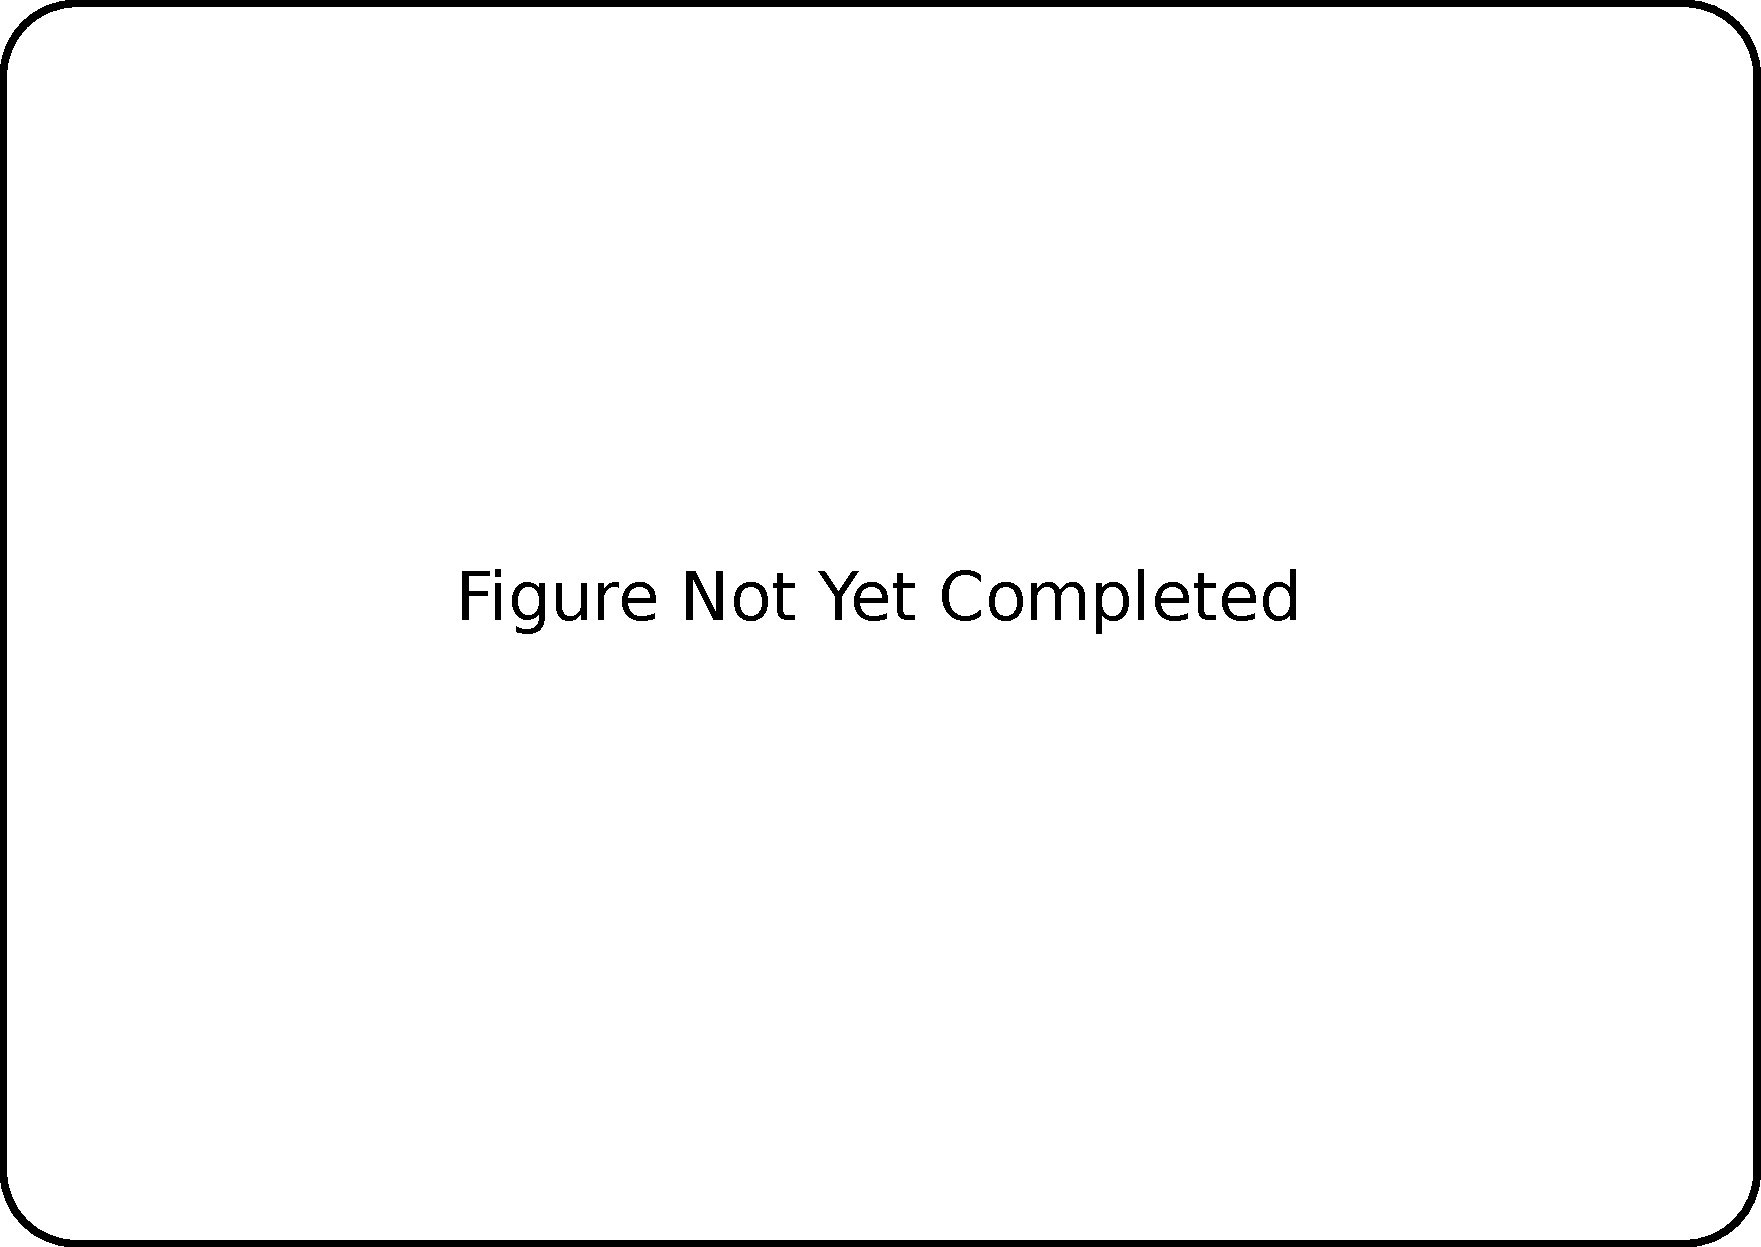
\includegraphics[width=4in]{introduction/not_finished.pdf}
%\end{center}
%\caption{Flow schematic for the PIC method with sceptic subroutine names Need to make figure}
%\label{fig:pic_flowchart_sceptic}
%\end{figure}


In the end the GPU implementation of SCEPTIC3D is very different from any other GPU PIC implementation. While we will focus a great deal on performance, we will also place a great deal of emphasis on implementation difficulty and applicability to future PIC implementations on the GPU. We will determine how critical the performance of the field solver is when the run time of other steps is significantly reduced. Lastly, we will look at how primarily graphics related GPU features can be utilized by PIC codes. 













